\section{O método simplex}\label{sec:metodo_simplex}
\subsection{Teoremas fundamentais para o método simplex}\label{sec:simplex pontos extremos}

\begin{mydef}[Reta]\label{def:reta}
Um poliedro $\vb P \subset \mathbb{R}^n$ contém uma \emph{reta} se existem um vetor $x \in \vb P$ e um vetor não-nulo $ d \in \mathbb{R}^n$ tais que $x + \lambda d \in \vb P$ para todo escalar $\lambda$.
\end{mydef}

\begin{theorem}\label{teo:retas}
    Suponha que o poliedro ${\vb P = \{x \in \mathbb{R}^n \mid a_i^\intercal x \leq b_i, i = 1,\ldots,m\}}$ é não-vazio. Então segue-se que:
    \begin{enumerate}[(a)]
    \item $\vb P$ tem pelo menos um ponto extremo.
    \item $\vb P$ não contém reta.
    \item Existem $n$ vetores da família $a_1,\ldots,a_m$ que são linearmente independentes.
    \end{enumerate}
\end{theorem}

\begin{proof}
    $(b) \Rightarrow (a)$

    Sejam $x \in \vb P$ e $ \vb I = \{i\mid a_i^\intercal x = b_i\}$. Se $n$ vetores $a_i, i \in  \vb I$, forem linearmente independentes, então $x$ é, por definição, uma solução básica factível e, portanto, existe ponto extremo em $\vb P$. Se este não for o caso, todos os vetores $ a_i, i \in  \vb I$, pertencem a um subespaço próprio de $\mathbb{R}^n$ e, destarte, existe um vetor $d \neq \vb 0$ tal que $a_i^\intercal d = 0$ para todo $i \in  \vb I$. Seja $y = x + \lambda  d$ uma reta, com $\lambda$ sendo um escalar arbitrário. Para $i \in  \vb I$, temos

    $$a_i^\intercal y = a_i^\intercal x + \lambda a_i^\intercal d = a_i^\intercal x = b_i.$$

    Logo, as restrições ativas em $ x$ permanecem ativas ao longo de toda a reta $ y$. Contudo, como estamos assumindo $(b)$ como hipótese, segue-se que, variando $\lambda$, estaremos eventualmente violando uma restrição. Na iminência de uma tal violação, uma nova restrição deve ficar ativa. Logo, existem $\lambda^*$ e $j \notin  \vb I$ tais que $a_j^\intercal (x + \lambda^*d) = b_j$.

    Vamos provar que $ a_j$ não é combinação linear dos vetores $ a_i, i \in  \vb I$. Temos que $a_j^\intercal x \neq b_j$ (pois $j \notin  \vb I$) e $a_j^\intercal (x + \lambda^*d) = b_j$ (pela definição de $\lambda^*$). Assim, $a_j^\intercal d \neq 0$. Por outro lado, $a_i^\intercal d = 0$ para todo $i \in  \vb I$ (pela definição de $ d$) e, portanto, $ d$ é ortogonal a qualquer combinação linear dos vetores $ a_i, i \in  \vb I$. Como $ d$ não é ortogonal a $ a_j$, concluímos que $ a_j$ não é combinação linear dos vetores $ a_i, i \in  \vb I$.

    Logo, no deslocamento do ponto $ x$ para $ x + \lambda^* d$, o número de restrições linearmente independentes aumenta em pelo menos um. Repetindo este argumento tantas vezes quanto for necessário, eventualmente chegamos a um ponto em que $n$ restrições são ativas. Por definição, este ponto é solução básica e, como não violamos nenhuma restrição, é solução básica factível e, portanto, um ponto extremo.

    $(a) \Rightarrow (c)$

    Se $x \in \vb P$ é ponto extremo, $ x$ também é solução básica factível, e existem $n$ restrições ativas em $ x$ cujos vetores $ a_i$ são linearmente independentes.

    $(c) \Rightarrow (b)$

    Suponha que $n$ dos vetores $ a_i$ sejam linearmente independentes e, sem perda de generalidade, sejam $a_1,\ldots,a_n$ linearmente independentes. Suponha que $\vb P$ contenha uma reta $ x + \lambda  d$, com $d \neq \vb 0$. Então, temos que $a_i^\intercal (x + \lambda d) \geq b_i$ para todo $i$ e todo $\lambda$. Concluímos que $a_i^\intercal d = 0$ para todo $i$. Como os vetores $ a_i, i = 1,\ldots,n$ são linearmente independentes, segue-se que $d = \vb 0$. Mas isso contradiz o que acabamos de definir para $ d$. Portanto, $\vb P$ não contém retas.
\end{proof}

Finalmente, estamos em condições de introduzir o teorema que justifica a ideia central do método simplex.

\begin{theorem}
    Considere o problema de otimização linear de minimizar $c^\intercal x$ em um poliedro $\vb P$. Suponha que $\vb P$ tenha pelo menos um ponto extremo. Então, ou o custo ótimo é igual a $-\infty$, ou existe um ponto extremo ótimo.
\end{theorem}

\begin{proof}
    Para esta demonstração, considere a seguinte terminologia: um elemento $x \in \vb P$ tem \emph{posto} $k$ se for possível encontrar $k$, e não mais que $k$, restrições linearmente independentes ativas em $x$.

    Suponha que o valor objetivo ótimo é finito. Seja $\vb P = \{x \in \mathbb{R}^n \mid Ax \leq b\}$ e considere $x \in \vb P$ com posto $k < n$. Vamos provar a existência de um $y \in \vb P$ com posto maior que $k$ que também satisfaça $c^\intercal y \leq c^\intercal x$. Seja $ \vb I = \{i\mid a_i^\intercal x = b_i\}$, onde $a_i^\intercal$ é a $i$-ésima linha de $ A$. Como $k < n$, os vetores $ a_i, i \in  \vb I$, pertencem a um subespaço próprio de $\mathbb{R}^n$, e podemos escolher um vetor $ d \in \mathbb{R}^n, d \neq \vb 0$, ortogonal a todo $ a_i, i \in  \vb I$. Ademais, considere que $ d$ é tal que $c^\intercal d \leq 0$.

    Suponha que $c^\intercal d < 0$ e considere a semirreta $y = x + \lambda  d$, onde $\lambda$ é um escalar positivo. Como se segue do \cref{teo:retas}, todos os pontos nesta semirreta satisfazem as relações ${a_i^\intercal y = b_i, i \in  \vb I}$. Se toda a semirreta estivesse contida em $\vb P$, o valor objetivo ótimo seria $-\infty$. Como esta não é nossa hipótese, concluímos que a semirreta sai de $\vb P$ a partir de algum ponto. Na iminência desta saída, temos $\lambda^* > 0$ e $j \notin  \vb I$ tais que $a_j^\intercal (x + \lambda^*d) = b_j$. Então, sendo $y = x + \lambda^* d$, vale que $c^\intercal y < c^\intercal x$. Consequentemente, como mostrado no teorema mencionado, $ a_j$ é linearmente independente em relação a $ a_i, i \in  \vb I$, e o posto de $ y$ é pelo menos $k + 1$.

    Agora suponha que $c^\intercal d = 0$. Seja $y = x + \lambda  d$ uma reta com $\lambda$ escalar arbitrário. Como $\vb P$ não contém retas, a reta precisa sair de $\vb P$ em algum ponto e, na iminência disso, temos outro vetor $ y$ de posto maior que $ x$. Ademais, como $c^\intercal d = 0$, temos $c^\intercal y = c^\intercal x$.

    Em ambos os casos, encontramos $ y$ tal que $c^\intercal y \leq c^\intercal x$ e $\mathrm{posto}( y) > \mathrm{posto}( x)$. Repetindo este processo quantas vezes for necessário, chegamos a um vetor $w$ tal que $\mathrm{posto}(w) = n$ e $c^\intercal w \leq c^\intercal x$.

    Sejam $w^1,\ldots,w^r$ as soluções básicas factíveis em $\vb P$ e seja $w^*$ uma solução básica factível tal que $c^\intercal w^* \leq c^\intercal w^i$ para todo $i$. Já demonstramos que para todo $ x$ existe $i$ tal que ${c^\intercal w^i \leq c^\intercal x}$. Segue-se que ${c^\intercal w^* \leq c^\intercal x}$ para todo $x \in \vb P$, e a solução básica factível $w^*$ é ótima.
\end{proof}

Note que se um poliedro não-vazio não tiver ponto extremo, sua solução ótima é $-\infty$. Pelo contrário, se o poliedro for não-vazio e tiver ponto extremo, sua solução ótima pode ser $-\infty$ ou está localizada em algum dos pontos extremos. Isso nos permite chegar à conclusão necessária para começar a desenvolver o método simplex.

\begin{cor}\label{cor:solução ótima}
Considere o problema de otimização linear de minimizar $c^\intercal x$ em um poliedro não-vazio. Então o custo ótimo é $-\infty$ ou existe solução ótima.
\end{cor}

Deste ponto em diante, chamaremos o caso em que a solução ótima do problema é $-\infty$ de \emph{caso ilimitado}.

\subsection{Considerações iniciais}

Agora que sabemos o exposto pelo \cref{cor:solução ótima}, podemos pensar em uma forma rudimentar de resolver problemas de otimização linear. Uma forma conceitualmente simples é descrita nos passos a seguir.

\begin{enumerate}
    \item Encontrar todas as soluções básicas $x^1,\ldots,x^p$.
    \item Determinar o conjunto $\vb{F} = \{x^i \mid x^i \text{ é factível}\}$.
    \item Encontrar o ponto ótimo $x^* = \min(\vb F)$.
\end{enumerate}

Evidentemente, esta abordagem tem problemas. Primeiramente, esta verificação não considera a possibilidade de a solução ótima ser $-\infty$. Além disso, como evidenciado pela \cref{eq:maxSBF}, existem $\binom{n}{m}$ maneiras de organizar as $n$ variáveis de decisão do problema de maneira que o sistema $\eqsys$ seja satisfeito junto com as restrições de não-negatividade; ou, ainda, existem $p = \binom{n}{m}$ soluções básicas para o problema. Logo, para problemas com número considerável de variáveis e restrições, este método é custoso já no primeiro passo, tornando-se praticamente inviável.

O método simplex implementa uma ideia mais sofisticada do exposto acima. Este método depende de um ponto extremo inicial e, a partir deste ponto, se desloca para um novo ponto extremo a cada iteração. O deslocamento do simplex é condicionado de modo que o método reduza o valor objetivo a cada iteração. Além disso, o método é capaz de determinar se o ponto em que se encontra é ótimo, ou se a solução ótima é $-\infty$, sem ter que compará-lo a todos os outros pontos extremos.

Implementamos o método simplex através de um pacote computacional chamado \texttt{Caique.jl} \cite{Centenaro:23}, que se encontra em um repositório do \emph{GitHub} (\url{https://github.com/phcentenaro7/Caique.jl}). O \texttt{Caique.jl} é um pacote escrito em Julia \cite{JULIA} que pode ser usado para resolver problemas de otimização linear. O código do pacote foi implementado com base nas obras de \textcite{BAZARAA:10,BERTSIMAS:97}, e põe em prática os algoritmos que serão apresentados nesta seção.

\emph{Caique} é o nome em inglês de uma espécie de pássaros conhecida no Brasil como marianinha. Como o método simplex "pula" de um ponto extremo do problema a outro, ele lembra bastante uma das muitas marianinhas saltitantes que podem ser encontradas em vídeos pela internet, servindo de inspiração para o nome do pacote.

\begin{figure}[h!]
    \centering
    \caption{Exemplo de marianinha \cite{BÉKÉSI:09}}
    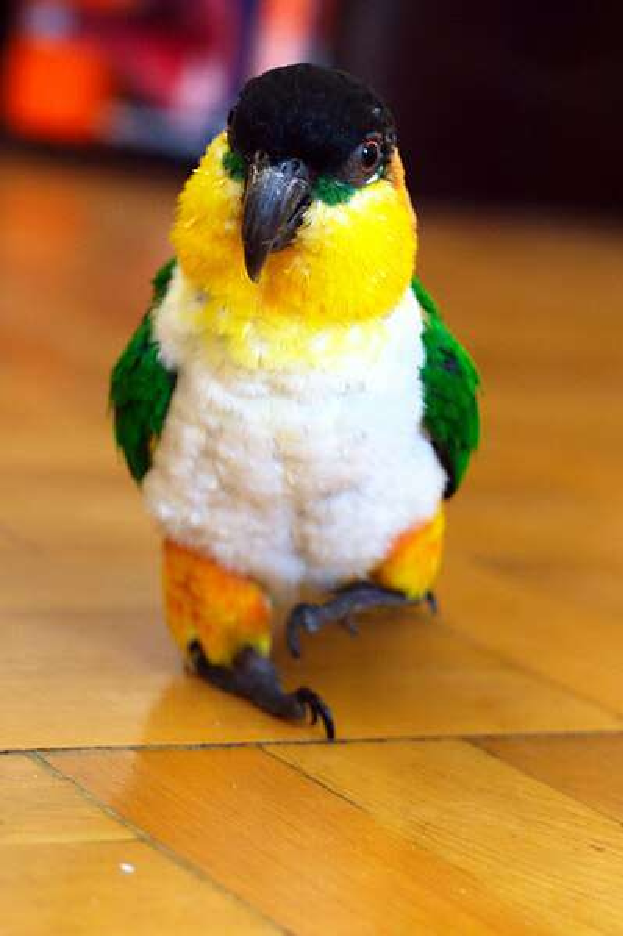
\includegraphics[scale=0.5]{imagens/marianinha.pdf}
\end{figure}


\subsection{Representação de um problema em forma canônica}\label{sec:forma canônica}

Antes de começar o desenvolvimento do simplex, precisamos garantir que o problema de otimização linear esteja na forma \emph{canônica}. Diferentemente da forma padrão, apresentada no \cref{eq:forma padrão}, a forma canônica se apresenta em termos apenas de igualdades, à exceção apenas das restrições de não-negatividade, que continuam as mesmas. O \cref{eq:forma canônica} apresenta a forma canônica.

\begin{align}\label[problem]{eq:forma canônica}
    \min\ &\objval\\
    \textrm{s.a }& \eqsys,\\
    &  x \geq \vb 0.
\end{align}

Neste caso, assim como na forma padrão, $A$ é uma matriz de dimensões $m\times n$, $\vc$ e $ x$ são vetores no $\mathbb{R}^{n}$ e $\vbb$ é um vetor no $\mathbb{R}^m$. 

É possível converter problemas da forma padrão para a forma canônica de modo que continuem os mesmos. Para tal, faremos uso de \emph{variáveis de folga}.

\begin{mydef}[Variável de folga]
    Dada uma restrição de desigualdade de um problema de otimização linear, uma nova variável $ x_s$ introduzida à restrição é definida como \emph{variável de folga} se:
    \begin{itemize}
        \item $a_i^\intercal x + x_s = b_i$, para $a_i^\intercal x \leq b_i$.
        \item $a_i^\intercal x - x_s = b_i$, para $a_i^\intercal x \geq b_i$.
    \end{itemize}
\end{mydef}

Note que, se adicionarmos uma variável de folga $ x_s$ à $i$-ésima restrição do problema, o vetor dos coeficientes de $ x_s$ para cada restrição será o $i$-ésimo vetor da base canônica, ou $ e_i$. Por outro lado, se subtrairmos $ x_s$ da restrição, então o vetor de coeficientes de $x_s$ será $- e_i$.

Usando variáveis de folga, podemos converter qualquer restrição de desigualdade em restrição de igualdade. Note que este processo gera um problema equivalente ao da forma padrão. A única diferença é que a variável representante da quantidade que falta para igualar os dois lados passa a ser explicitada.

Por razões que veremos no \cref{sec:duas fases}, é importante garantir que o vetor de valores do lado direito das equações, $b$, seja não-negativo. Sendo $i = 1,\ldots,m$, isso pode ser feito multiplicando por $-1$ as equações para as quais $ b_i < 0$. Equivalentemente, podemos multiplicar as inequações ainda no formato padrão do problema por $-1$.

A implementação do procedimento que permite a conversão de um problema para a forma canônica é feita no \href{https://github.com/phcentenaro7/Caique.jl}{\texttt{Caique.jl}}, na função 
\href{https://github.com/phcentenaro7/Caique.jl/blob/9c78027f1884181846a6321a5640f92c9a718ce4/src/LinearProgram.jl#L41}{\julia{createSlackSubmatrix}}, nos moldes do \cref{alg:variáveis de folga}. No código, existe a estrutura imutável \href{https://github.com/phcentenaro7/Caique.jl/blob/main/src/LinearProgram.jl}{\julia{LinearProgram}}, que recebe, como argumentos para sua construção, a matriz $ A$ e os vetores $b, c, x$ e, ainda, um vetor $s$, que contém valores conhecidos na linguagem como \emph{símbolos}. Um símbolo é uma sucessão de caracteres, sem espaços, precedida por dois pontos. No caso, usamos o vetor de símbolos $s$ para definir se as restrições que estão sendo passadas ao construtor são de igualdade, maior igual ou menor igual (\julia{:equal}, \julia{:greater} e \julia{:less} na implementação, respectivamente). Para adicionar as variáveis de folga ao problema, o objetivo é criar uma matriz $ X^s$ que represente a adição ou subtração das variáveis de folga necessárias. Esta matriz pode ser concatenada à direita da matriz $ A$, de modo que a nova matriz $ A$ passe a representar também as variáveis de folga.

Note que, a partir daqui, estaremos nos referindo à $i$-ésima linha de uma matriz $A$ qualquer por $ A_i$, e à $i$-ésima coluna desta matriz por $a_i$, por simplicidade de notação.

\begin{algorithm}
\begin{algorithmic}[1]
\caption{Adicionar variáveis de folga ao problema (\href{https://github.com/phcentenaro7/Caique.jl/blob/9c78027f1884181846a6321a5640f92c9a718ce4/src/LinearProgram.jl\#L41}{Implementação})}\label{alg:variáveis de folga}
\State criar uma matriz $ X^s$ de dimensões $m\times0$, que representa as restrições das variáveis de folga
\State definir $i \gets 1$, que será nosso contador de linhas
\State definir $k \gets 1$, que será o contador do número de variáveis de folga adicionadas ao problema
\While{$i \leq m$}
    \If{$ b_i < 0$}
        \State redefinir o valor do lado direito $ b_i \gets -( b_i)$
        \State redefinir a linha $A_i \gets -A_i$
        \State inverter o sinal da restrição, se for uma inequação
    \EndIf
    \If{o sinal da restrição for $\leq$}
        \State redefinir $k \gets k + 1$
        \State redefinir $x_S \gets [x_S, e_i]$
    \ElsIf{o sinal da restrição for $\geq$}
        \State redefinir $k \gets k + 1$
        \State redefinir $x_S \gets [x_S, -e_i]$
\EndIf
\State redefinir $i \gets i + 1$
\EndWhile
\State Concatenar $k$ zeros ao vetor de custos, um para cada variável de folga adicionada ao problema
\State \Return a matriz $ X^s$ atual, pois chegamos ao fim do algoritmo
\end{algorithmic}
\end{algorithm}

Após o término deste algoritmo, a matriz $ X^s$ pode ser concatenada à direita da matriz $ A$, produzindo a representação em forma canônica do problema, como desejado.

\subsection{Variáveis básicas e não-básicas}\label{sec: x_B e  x_N}

Como explicado na introdução desta seção, para que o método simplex funcione, precisamos começar o problema em uma solução básica factível. Note, pela \cref{def:sbf}, que, para que um ponto seja solução básica factível, ele precisa, entre outras coisas, ter $n$ restrições linearmente independentes ativas nele. Neste trabalho, vamos considerar um problema de otimização linear na forma canônica com $\text{posto}( A) = m$. Então, segue-se que $n \geq m$. O que nos interessa é o caso não-trivial em que $n > m$. Note que podemos encontrar uma solução básica seguindo os passos a seguir.

\begin{enumerate}
    \item Zerar $n - m$ das variáveis de decisão do problema.
    \item Resolver o sistema de equações $Ax = b$.
\end{enumerate}

Note que, ao fixar $n - m$ variáveis de decisão em zero, sobram $m$ variáveis para resolver um sistema de $m$ equações. Ou seja, os dois passos acima nos permitem trivialmente encontrar soluções básicas, bastando permutar as variáveis que definimos como zero. Note, ainda, que isso não nos garante que a solução básica encontrada seja \emph{factível}; ou seja, pode ser que, com as variáveis que escolhemos zerar, o sistema de equações $Ax=b$ não resulte em $x \geq \vb 0$.

Para problemas pequenos, é possível permutar soluções básicas até que se verifique que uma delas é factível; no entanto, como mostrado pela \cref{eq:maxSBF}, este procedimento é computacionalmente inviável para problemas grandes. Como veremos adiante, é possível definir um novo problema de otimização linear a partir do original que, fornecido ao método simplex, pode nos retornar uma solução básica factível para o problema original. Todavia, isso requer que primeiro desenvolvamos o método simplex. Então vamos supor, por ora, que sempre temos uma solução básica factível pela qual começar.

Agora que temos um método para obter soluções básicas, é útil definir termos muito importantes para desenvolvimento do método simplex. Sendo $ x$ o vetor de variáveis de decisão do problema de otimização linear, valem as seguintes definições.

\begin{mydef}[Variável não-básica]
    Uma variável $ x_i, i \in \{1,\ldots,m\}$, é dita \emph{não-básica} quando $ x_i = 0$ para satisfazer uma das restrições de não-negatividade do problema.
\end{mydef}

\begin{mydef}[Variável básica]
    Uma variável $ x_i, i \in \{1,\ldots,m\}$, é dita \emph{básica} quando ela constitui solução do problema $\eqsys$ após a seleção das variáveis não-básicas.
\end{mydef}

\begin{mydef}[Matriz base]
    Assuma, sem perda de generalidade, que as variáveis básicas do problema tenham índices $1,\ldots,m$. Então a \emph{matriz base} do problema é definida como $ B = [a_1,\ldots,a_m]$. 
\end{mydef}

\begin{mydef}[Matriz não-base]
    Assuma, sem perda de generalidade, que as variáveis não-básicas do problema tenham índices $m+1,\ldots,n$. Então a \emph{matriz não-base} do problema é definida como $ N = [a_{m+1},\ldots,a_n]$.
\end{mydef}

Feitas estas definições, podemos reescrever o \cref{eq:forma canônica} como

\begin{align}\label[problem]{eq:forma canônica xBxN}
    \min\ &{ c_B\ip  x_B + \vcN\ip  x_N}\\
    \text{s. a\ }& B  x_B +  N  x_N = \vbb,\\
    &   x_B,   x_N \geq \vb 0,
\end{align}
onde $ B$ é a matriz base, $ N$ é a matriz não-base, $  x_B$ é o vetor de variáveis básicas e $  x_N$ é o vetor de variáveis não-básicas.

Por fim, introduzimos o conceito de degeneração em poliedros, que é uma extensão da \cref{def:degeneração}.

\begin{mydef}[Degeneração em poliedros]
    Considere o poliedro na forma canônica ${\vb P = \{ x \in \mathbb{R}^n \mid \vA x = \vbb,  x \geq \vb 0\}}$, sendo $ x$ solução básica. Seja $\vA$ uma matriz $m\times n$. O vetor $ x$ é uma solução básica \emph{degenerada} se o número de componentes nulos de $ x$ for maior do que $n - m$.
\end{mydef}

Da maneira como estamos construindo soluções básicas, só é possível uma destas soluções ser degenerada se uma das variáveis básicas tiver que ser igual a zero para resolver $\eqsys$. Neste caso, além das $n$ restrições ativas esperadas, surgem $k$ restrições de não-negatividade ativas a mais do que o esperado, para $k$ variáveis básicas iguais a zero. Assim, a solução básica em questão será ativa em $n + k$ restrições. Como estamos no $\mathbb{R}^n$, isso significa que $k$ restrições ativas são linearmente dependentes em relação às demais.

Como veremos no \cref{sec:degeneração}, pontos degenerados podem travar o método simplex no lugar, requerendo métodos especiais para superá-los.

\subsection{Mecanismo iterativo de redução do valor objetivo}\label{sec:mecanismo simplex}

Nosso objetivo agora é verificar como o simplex garante que o valor objetivo é reduzido de uma iteração para a outra. Podemos continuar decompondo o \cref{eq:forma canônica xBxN} para chegar aonde queremos.

Começamos pré-multiplicando ambos os lados do sistema de equações pela inversa da base, obtendo

\begin{equation}\label{eq:vezes inversa}
      x_B + \invB N  x_N = \invB\vbb.
\end{equation}

Denotando por $j_{(1)},\ldots,j_{(n-m)}$ os índices das variáveis não-básicas, note que

\begin{align}
     N  x_N &=
    \begin{bmatrix}
    a_{j(1)} && \ldots && a_{j(n-m)}
    \end{bmatrix}
    \begin{bmatrix}
        x_{j(1)}\\
        \vdots\\
        x_{j(n-m)}
    \end{bmatrix}\\
    &= (a_{j(1)}x_{j(1)} + \dots + a_{j(n-m)}x_{j(n-m)}).
\end{align}

Ou seja, sendo $ \vb J$ o conjunto de índices das variáveis não-básicas do problema, podemos escrever

\begin{equation}
    \invB N  x_N = \invB\sum_{j\in J}{ a_j x_j} = \sum_{j\in J}{\invB a_j x_j}.
\end{equation}

Agora vamos definir $\vbbbar = \invB\vbb$ e reescrever a equação em termos do conjunto $ \vb J$:

\begin{equation}
      x_B + \sum_{j\in \vb J}{\invB a_j x_j} = \vbbbar.
\end{equation}

Seja $y_j = B^{-1}a_j, j \in \vb J$. Então, substituindo os termos na equação e isolando $  x_B$, temos:

\begin{equation}
      x_B = \vbbbar - \sum_{j\in \vb J}{y_j x_j}.
\end{equation}

Note que isso nos permite reescrever a expressão da função objetivo do \cref{eq:forma canônica xBxN} como

\begin{equation}
    z =  c_B\ip\left(\vbbbar - \sum_{j\in \vb J}{y_j x_j}\right) + \sum_{j\in \vb J} c_j x_j,
\end{equation}
onde $ c_B$ é o vetor de custos das variáveis básicas.

Considere $z_0 =  c_B\ip\vbbbar$ e $ z_j =  c_B\ip y_j$. Então ficamos com

\begin{equation}
    z = z_0 - \sum_{j\in \vb J}{ z_j x_j} + \sum_{j\in \vb J} c_j x_j.
\end{equation}

Por fim, podemos unir as expressões dos somatórios como

\begin{equation}
    z = z_0 - \sum_{j\in \vb J}{(z_j - c_j)} x_j,
\end{equation}
e podemos simplificar a expressão considerando $\bar{ z_j} = z_j - c_j$:

\begin{equation}
    z = z_0 - \sum_{j\in \vb J}{\bar{ z_j}} x_j.
\end{equation}

O \cref{eq:pl reescrito} mostra o resultado da nova representação do \cref{eq:forma canônica xBxN}.

\begin{align}\label[problem]{eq:pl reescrito}
    \min\ &z_0 - \sum_{j\in \vb J}{\bar{ z_j}} x_j\\
    \text{s. a }&  x_B + \sum_{j\in \vb J}{ y_j x_j} = \vbbbar,\\
    &   x_B,   x_N \geq \vb 0.
\end{align}

Perceba que reescrevemos o problema de modo que as variáveis básicas passaram a cumprir papel de variáveis de folga. Ou seja, nesta representação, as variáveis básicas aparecem uma única vez, em restrições diferentes. Isso é excelente para o método simplex, pois nos permite obter facilmente os valores de $  x_B$ conforme $  x_N$ varia.

Para entender este ponto, vamos imaginar que estejamos em uma solução básica factível. Então, segue-se que $  x_N = \vb 0$ e, portanto, $  x_B = \vbbbar$. Além disso, $z = z_0$. Disso tiramos que $z_0$ é o valor objetivo do problema na solução atual.

Agora imagine que queiramos reduzir o valor objetivo. Evidentemente, isso pode ser feito aumentando o valor de um variável não-básica $ x_k$, para a qual $\bar{ z_k} > 0$. Se não existir $k$ tal que $\bar{ z_k}$ satisfaça esta condição, então o ponto atual é ótimo. Do contrário, geralmente é mais interessante escolher $ x_k$ para a qual $\bar{ z_k}$ seja máximo, pois então a redução unitária do valor objetivo é a maior possível. Qualquer que seja a variável escolhida para ter seu valor aumentado, passamos a chamá-la de \emph{variável de entrada}. Para entender este nome, vamos analisar o que acontece quando escolhemos aumentar o valor da variável $ x_k$. Isolando $  x_B$ no \cref{eq:pl reescrito}, temos

\begin{equation}\label{eq:base na troca}
      x_B = \vbbbar - { y_k x_k}.
\end{equation}

Em particular, imagine uma variável básica de índice $r$ para a qual $y_{kr} > 0$. Segue-se que, quanto mais o valor de $ x_k$ for aumentado, mais $ x_r$ diminuirá. Esta diminuição só pode ocorrer até que $ x_r = 0$, pois, do contrário, $ x_r$ estará violando sua restrição de não-negatividade.

Imagine agora que $ x_r$ seja a primeira variável que fica igual a zero quando $ x_k$ aumenta, ou seja, $ x_r$ define quando o crescimento de $ x_k$ deve parar e, por isso, $ x_r$ é chamada de \emph{variável de bloqueio}. Perceba que, quando isso acontece, $ x_k$ vira variável básica e $ x_r$ vira variável não-básica. Por isso, a variável de bloqueio também é conhecida como \emph{variável de saída}, e dizemos que $ x_k$ \emph{entra} na base e $ x_r$ \emph{sai} da base.

Feito este raciocínio, sabemos que o valor de $ x_k$ após a detecção da variável de bloqueio será

\begin{equation}\label{eq:xNk}
     x_k = \frac{\bar{b_r}}{y_{kr}}.
\end{equation}

Note que as alterações que as variáveis básicas sofrem não alteram o valor objetivo, e note também que $ x$ continua satisfazendo $n$ restrições linearmente independentes. Portanto, o ponto para o qual nos deslocamos é vértice. Mais especificamente, como tudo que fizemos foi trocar a restrição de não-negatividade ativa, realizamos um deslocamento até uma solução básica factível adjacente.

Por fim, suponha que $ y_k \leq 0$. Neste caso, note que $ x_k$ reduz o valor do lado esquerdo de todas as restrições do \cref{eq:pl reescrito} nas quais ele aparece. Assim, as variáveis básicas aumentarão nas proporções necessárias para garantir que o sistema de equações continue sendo satisfeito. Todas as demais variáveis continuam respeitando as restrições de não-negatividade e, portanto, temos a garantia de que estamos em um ponto factível, qualquer que seja o valor para o qual aumentarmos $ x_k$. Logo, quando $ x_k \to \infty$, sabemos que $z \to -\infty$, e concluímos que a semirreta

\begin{equation}\label[ray]{eq:semirreta ótima}
    \left[\begin{array}{c}
          x_B\\
        \vb{0}
    \end{array}\right]
    +
    \left[\begin{array}{c}
        - y_k\\
         e_k
    \end{array}\right]
     x_k
\end{equation}
indica um sentido de redução infinita do valor objetivo do problema. Com isso, provamos que o método simplex é capaz de determinar se um problema tem caso ilimitado.

\subsection{Uma formulação inicial do simplex}\label{sec:formulação simplex}

Agora que conhecemos o mecanismo iterativo do simplex, estamos habilitados a descrever o método em forma de passo a passo. Na sua forma mais simples, o simplex pode ser descrito como o \cref{alg:simplex}.

\begin{algorithm}
\begin{algorithmic}[1]
    \floatname{algorithm}{Método}
    \caption{Simplex (\href{https://github.com/phcentenaro7/Caique.jl/blob/9c78027f1884181846a6321a5640f92c9a718ce4/src/Simplex.jl\#L36}{Implementação})}\label[method]{alg:simplex}
    \State definir $\text{iter} \gets 1$ como o número de iterações
    \State definir $\text{maxiter}$ como o número máximo de iterações
    \While{a solução ótima for desconhecida e $\text{iter} < \text{maxiter}$}
        \State realizar a \emph{atualização das variáveis}
        \State realizar a operação de \emph{precificação} e \Return o ponto ótimo, se existir
        \State realizar o \emph{teste do caso ilimitado} e \Return a semirreta ótima, se existir
        \State realizar o \emph{teste da razão mínima}
        \State trocar as variáveis de entrada e de saída
        \State redefinir $\text{iter} \gets \text{iter} + 1$
    \EndWhile
    \State \Return que o número máximo de iterações foi atingido sem encontrar uma solução
\end{algorithmic}
\end{algorithm}

Vamos discutir os passos principais em mais detalhes a seguir.

\subsubsection*{Atualização das variáveis}
Como o simplex lida com pontos extremos do problema de otimização linear, segue-se que a cada iteração precisamos, no mínimo, de dados que descrevam quais são os valores atuais das variáveis básicas, qual é a matriz base e qual é o valor objetivo do problema. Assim, o passo de atualização das variáveis pode ser formulado como no \cref{alg:atualização das variáveis}.

\begin{algorithm}
\begin{algorithmic}[1]
    \caption{Atualização das variáveis (\href{https://github.com/phcentenaro7/Caique.jl/blob/9c78027f1884181846a6321a5640f92c9a718ce4/src/Simplex.jl\#L80}{Implementação})}\label{alg:atualização das variáveis}
    \State atualizar a matriz base $ B \gets [a_{i(1)}, \ldots, a_{i(m)}]$, onde $i(1), \ldots, i(m)$ são os índices das variáveis básicas
    \State atualizar os valores das variáveis básicas $  x_B \gets B^{-1}b$
    \State atualizar $\vbbbar \gets   x_B$
    \State atualizar o valor objetivo $z \gets \vc\ip  x_B$
\end{algorithmic}
\end{algorithm}

A partir deste conjunto simples de dados, todos os demais passos de uma iteração do método simplex funcionam.\footnote{No \texttt{Caique.jl}, aproveitamos a \emph{fatoração LU} \cite{UFRGS:LU} do Julia para otimizar operações que envolvam a matriz base. Assim, a matriz base (\julia{B}) serve apenas como uma forma de chegar à sua fatoração LU (\julia{Blu}), podendo ser descartada em seguida.}

\subsubsection*{Precificação}
A precificação é o processo preliminar para a seleção de uma variável de entrada, discutida no \cref{sec:mecanismo simplex}. O \cref{alg:precificação} descreve este processo.

\begin{algorithm}
\begin{algorithmic}[1]
    \caption{Precificação (\href{https://github.com/phcentenaro7/Caique.jl/blob/9c78027f1884181846a6321a5640f92c9a718ce4/src/Simplex.jl\#L88}{Implementação})}\label{alg:precificação}
    \State definir $ w \gets  c_B\ip\invB$, conhecido como \emph{vetor de multiplicadores simplex}
    \State definir a matriz não-base como $ N \gets [a_{j(1)}, \ldots, a_{j(m)}]$, onde $j(1), \ldots, j(m)$ são os índices das variáveis não-básicas
    \State definir o vetor de reduções unitárias de custo $\bar{ z} \gets  N\ip w - c_N$
    \State obter a variável não-básica $ x_k$ tal que $\zbar{k} = \max(\bar{ z})$
    \If{$\zbar{k} \leq 0$}
        \State \Return a solução atual, pois ela é ótima
    \EndIf
    \State \Return o índice $k$ da variável de entrada
\end{algorithmic}
\end{algorithm}

Se a precificação não retornar ponto ótimo, então temos uma variável não-básica $ x_k$ com potencial para entrar na base.

\subsubsection*{Teste de caso ilimitado}
Quando a precificação não retorna ponto ótimo, devemos verificar a possibilidade de que $ x$ seja o vértice de uma semirreta que leva a solução ótima a $-\infty$. Este teste é descrito no \cref{alg:teste de caso ilimitado}.

\begin{algorithm}
\begin{algorithmic}[1]
    \caption{Teste de caso ilimitado (\href{https://github.com/phcentenaro7/Caique.jl/blob/9c78027f1884181846a6321a5640f92c9a718ce4/src/Simplex.jl\#L127}{Implementação})}\label{alg:teste de caso ilimitado}
    \State definir $ y_k \gets B^{-1}a_k$
    \State obter $y_{k*} \gets \max( y_k)$
    \If{$y_{k*} \leq 0$}
        \State \Return a \cref{eq:semirreta ótima}, pois a solução atual é vértice da semirreta, que descreve a direção na qual a solução ótima tende a $-\infty$
    \EndIf
\end{algorithmic}
\end{algorithm}

\subsubsection*{Teste da razão mínima}
No caso de os dois algoritmos anteriores não terem retornado solução ótima, concluímos que ainda é possível realizar uma otimização finita do valor objetivo. Pela \cref{eq:xNk}, note que

\begin{equation}\label{eq:min ratio test}
     x_k = \min_{1\leq i \leq m}\left\{\frac{\bar{ b_i}}{y_{ik}}, y_{ik} > 0 \right\}
\end{equation}
deve ser o valor da variável de entrada, com o índice $r$ da variável de saída igual ao $i$ para o qual a \cref{eq:min ratio test} é mínima.

Esta maneira de encontrar a variável de saída é conhecida como teste da razão mínima. O \cref{alg:min ratio test} expressa uma forma de implementá-la.\footnote{É importante destacar que existem várias maneiras de implementar a checagem da variável de saída. Apesar de a lógica matemática indicar que devemos ignorar todos os $y_{ik} \leq 0$, a lógica de programação pode seguir um caminho diferente. No caso do \texttt{Caique.jl}, aproveitamos a alta abstração de Julia para definir todas as razões com $y_{ik} \leq 0$ como $\infty$ (ou \julia{Inf}, na terminologia do Julia). Isso facilita a obtenção do índice $r$, mas ao custo de mais memória.}

\begin{algorithm}[t]
\begin{algorithmic}[1]
    \caption{Teste da razão mínima (\href{https://github.com/phcentenaro7/Caique.jl/blob/9c78027f1884181846a6321a5640f92c9a718ce4/src/Simplex.jl\#L153}{Implementação})}\label{alg:min ratio test}
    \State definir um vetor vazio $ q$ de razões
    \State definir $i \gets 1$
    \While{$i \leq m$}
        \If{$\yik \leq 0$}
            \State ignorar $\ratio$
        \Else
            \State concatenar $\ratio$ ao vetor $ q$
        \EndIf
    \EndWhile
    \State \Return a variável de saída $r$ tal que $\minratio$ é o menor valor do vetor $ q$
\end{algorithmic}
\end{algorithm}

Com isso, definimos todo o método simplex na sua forma mais básica. Mas esta forma tem limitações consideráveis. Por exemplo, ainda não desenvolvemos um método para obter uma solução básica factível inicial que não recorra a força bruta ou a um palpite. Nosso método também é inútil caso encontre um ponto degenerado durante a resolução de um problema.

Apesar das limitações, esta versão do simplex pode ser modificada de modo a solucionar todos estes problemas. É isso que abordaremos depois que provarmos que o método desenvolvido converge para uma solução ótima em um número finito de iterações.

\subsubsection*{Prova de convergência finita}
\begin{theorem}
    Na ausência de degeneração, o método simplex termina em um número finito de iterações, com a conclusão de que existe uma solução básica factível ótima ou que o valor objetivo ótimo é $-\infty$.
\end{theorem}
\begin{proof}
    Em cada iteração, ocorre uma de três coisas:
    \begin{enumerate}[(a)]
        \item Para-se em uma solução básica factível ótima, quando $\bar{ z_k} \leq \vb{0}$.
        \item Para-se no vértice de uma solução ilimitada, quando $\bar{ z_k} > \vb{0}$ e $ y_k \leq \vb 0$.
        \item É obtida uma nova solução básica factível de valor objetivo reduzido, quando $\bar{ z_k} > \vb 0$ e $ y_k \nleq \vb 0$.
    \end{enumerate}
    Pelo item (c), concluímos que, de uma iteração para outra, o método simplex se desloca para uma solução básica factível diferente, sem repetições. Além disso, pelo \cref{teo:SBFs finitas}, existe um número finito de soluções básicas factíveis. Logo, o método simplex encontra um ponto que satisfaça (a) ou (b) em um número finito de iterações. 
\end{proof}

\subsection{O simplex tableau}
O método desenvolvido na subseção anterior é difícil de acompanhar. Perceba que só mantemos os valores relevantes para uma variável não-básica na memória -- a variável de entrada. De resto, não sabemos que mudanças estão acontecendo. Não sabemos quais outras variáveis tinham potencial de entrar na base, nem de que maneira a escolha da variável de entrada afetou as demais.

Precisamos de outra maneira de representar -- ou mesmo de pensar -- o simplex para poder entender melhor o que acontece a cada iteração. Não à toa, para discutir conceitos mais avançados sobre o método, costuma-se apresentá-lo em formato de tableau \cite{BERTSIMAS:97}.

\subsubsection{Construção do tableau inicial}\label{sec:construção tableau}

Existem múltiplas formas de apresentar o simplex tableau, mas seguiremos a usada por Bazaraa, Jarvis e Sherali \cite{BAZARAA:10}. Sem perda de generalidade, suponha que as variáveis básicas estão organizadas com os índices $1,\ldots,m$, enquanto as variáveis não-básicas estão organizadas com os índices $m+1,\ldots,n$. Então construímos o tableau do modo indicado a seguir.

\begin{table}[ht]
    \centering
    \setlength{\tabcolsep}{12pt}
    \renewcommand{\arraystretch}{1.5}
    \begin{tabular}{c|c|ccc|ccc|c|}
        \mc{} & \mc{$z$} & \mc{$x_1$} & \mc{$\dots$} & \mc{$x_m$} & \mc{$x_{m+1}$} & \mc{$\dots$} & \mc{$x_n$} & \mc{RHS}\\
        \cline{2-9}
        $z$ & 1 & 0 & $\dots$ & 0 & $\bar{z}_{m+1}$ & $\dots$ & $\bar{z_n}$ & $\vc\ip\vbbbar$ \\
        \cline{2-9}
        $x_1$ & 0 & & & & & & & \\
        $\vdots$ & $\vdots$ & & $\vb I$ & & & $B^{-1}N$ & & $\vbbbar$ \\
        $x_m$ & 0 & & & & & & & \\
        \cline{2-9}
    \end{tabular}
    \caption{}\label{tab:tableau trivial}
\end{table}

A partir daqui, vamos chamar a linha de $z$ de linha zero e a coluna de $z$ de coluna zero. Note que, em termos das variáveis não-básicas, a linha zero contém todos os respectivos coeficientes de redução unitária do valor objetivo. Já para as linhas $1,\ldots,m$, remonte à \cref{eq:vezes inversa}. Perceba que estas linhas mostram os valores dos coeficientes das variáveis não-básicas nas restrições de igualdade da nova representação do problema. Isso também explica por que as linhas $1,\ldots,m$ das variáveis básicas formam uma matriz identidade -- afinal, como discutido logo após a apresentação do \cref{eq:pl reescrito}, as variáveis básicas atuam como variáveis de folga (ver discussão sobre variáveis de folga no \cref{sec:forma canônica}).

Quanto à linha zero das variáveis básicas, chegamos à conclusão de que é preenchida por zeros através de uma conta simples. Suponha uma variável básica $ x_i, i \in \{1,\ldots,m\}$. Então a expressão da sua redução unitária de valor objetivo é

\begin{equation}
    \bar{z_i} = z_i -  c_i =  c_B\ip\invB  a_i -  c_i.
\end{equation}

Lembre-se que $ B = [a_1,\ldots,a_i,\ldots,a_m]$ e $\invB B = \vb I = [e_1,\ldots,e_i,\ldots,e_m]$. Para uma mesma coluna $ a_i$, as linhas serão definidas pelo produto das linhas $1,\ldots,m$ de $\invB$ com $ a_i$. Ou seja, as demais colunas de $ B$ são irrelevantes para a determinação do vetor resultante, e podemos concluir que $B^{-1}a_i = e_i$. Logo,

\begin{equation}
    \bar{z_i} =  c_B\ip e_i -  c_i.
\end{equation}

Mas $ c_B\ip e_i =  c_i$. Portanto, $\bar{z_i} = 0$ para todas as variáveis básicas.

A coluna RHS (\emph{right-hand-side}) apresenta os valores da função objetivo e das variáveis básicas na iteração. Já a coluna $z$ expressa o mesmo que a linha zero, exceto pela ausência de variáveis não-básicas. Com isso, descrevemos toda a estrutura do tableau. Perceba que tudo que envolve as variáveis básicas é obtido trivialmente e que a coluna $z$ é sempre a mesma.

A \cref{tab:tableau generalizado} mostra outra representação possível para uma construção inicial do simplex tableau, sem considerar as trivialidades expostas pela \cref{tab:tableau trivial}.

\begin{table}[ht]
    \centering
    \setlength{\tabcolsep}{12pt}
    \renewcommand{\arraystretch}{1.5}
    \caption{}\label{tab:tableau generalizado}
    \begin{tabular}{c|c|ccc|c|}
        \mc{} & \mc{$z$} & \mc{$x_1$} & \mc{$\dots$} & \mc{$x_n$} & \mc{RHS}\\
        \cline{2-6}
        $z$ & 1 & $\bar{z}_1$ & $\dots$ & $\bar{z_n}$ & $\vc\ip\vbbbar$ \\
        \cline{2-6}
        $x_1$ & 0 & & & & \\
        $\vdots$ & $\vdots$ & & $B^{-1}A$ & & $\vbbbar$ \\
        $x_m$ & 0 & & & & \\
        \cline{2-6}
    \end{tabular}
\end{table}

\subsubsection{Cálculo de nova iteração por pivoteamento}\label{sec:pivoteamento tableau}
Podemos iterar o simplex tableau por meio de operações matriciais de pivoteamento. Nesta subseção, vamos enunciar e desenvolver todos os passos que justificam o pivoteamento do simplex.

Sejam $k$ o índice da variável de entrada e $r$ o índice da variável de saída. Então o coeficiente $y_{rk}$ é chamado de \emph{pivô} do método simplex. No simplex tableau, $y_{rk}$ pode ser encontrado na linha $r$, coluna $k$, como mostra a \cref{tab:pivô}.

\begin{table}[ht]
    \centering
    \setlength{\tabcolsep}{18pt}
    \renewcommand{\arraystretch}{2}
    \caption{}\label{tab:pivô}
    \begin{tabular}{c|c|ccccc|c|}
        \mc{} & \mc{$z$} & \mc{$x_1$} & \mc{$\dots$} & \mc{$x_{k}$} & \mc{$\dots$} & \mc{$x_n$} & \mc{RHS}\\
        \cline{2-8}
        $z$ & 1 & $\zbar{1}$ & $\dots$ & $\zbar{k}$ & $\dots$ & $\zbar{n}$ & $\vc\ip\vbbbar$ \\
        \cline{2-8}
        $x_1$ & 0 & $ y_{11}$ & $\dots$ & $ y_{1k}$ & $\dots$ & $ y_{1n}$ & $\bar{b_1}$ \\
        $\vdots$ & $\vdots$ & $\vdots$ & $\ddots$ & $\vdots$ & $\ddots$ & $\vdots$ & $\vdots$ \\
        $ x_r$ & 0 & $ y_{r1}$ & $\dots$ & \circled{$ y_{rk}$} & $\dots$ & $ y_{rn}$ & $\bar{b_r}$\\
        $\vdots$ & $\vdots$ & $\vdots$ & $\ddots$ & $\vdots$ & $\ddots$ & $\vdots$ & $\vdots$ \\
        $x_m$ & 0 & $ y_{m1}$ & $\dots$ & $ y_{mk}$ & $\dots$ & $ y_{mn}$ & $\bar{b_m}$\\
        \cline{2-8}
    \end{tabular}
\end{table}

Dito isso, o pivoteamento do simplex é feito através do \cref{alg:pivoteamento simplex}.

\begin{algorithm}
\begin{algorithmic}[1]
\caption{Pivoteamento do simplex}\label{alg:pivoteamento simplex}
    \State Dividir a linha $r$ por $ y_{rk}$.
    \State Para todo $t \in \{1,\ldots,m\}\setminus\{r\}$, atualizar a $t$-ésima linha subtraindo dela $ y_{tk}$ vezes a nova $r$-ésima linha.
    \State Atualizar a linha zero subtraindo dela $\zbar{k}$ vezes a nova $r$-ésima linha.    
\end{algorithmic}
\end{algorithm}

Agora vamos justificar cada um dos passos do pivoteamento. A princípio, perceba que a intenção do pivoteamento é transformar $x_{k}$ em variável básica. Como o \cref{eq:pl reescrito} organiza todas as variáveis básicas na forma de variáveis de folga, nosso objetivo é fazer com que $x_{k}$ apareça com coeficiente $1$ na linha $r$ do tableau e $0$ em todas as demais. Note que estamos incluindo a linha zero, pois, como mostrado no \cref{sec:construção tableau}, o valor de $x_{k}$ nesta linha deverá ser zero. Evidentemente, como consequência de estarmos rearranjando o problema, as demais variáveis também terão seus coeficientes alterados de modo a manter as igualdades entre os lados. Esclarecido o objetivo do pivoteamento, sigamos para as justificações.

\textbf{Passo 1}

Queremos que $x_{k}$ tenha coeficiente $1$ na linha $r$. A razão para tal é simples: $x_{r}$ é a única variável básica na restrição $r$. Para que a igualdade continue sendo possível, segue-se que $x_{k}$ precisa substituir $x_{r}$ nesta restrição.

Seja $ \vb I = \{1,\ldots,m\}$. Então note que a restrição $r$ pode ser equacionada como

\begin{equation}\label{eq:r-ésima linha tabela}
    \sum_{\substack{i \in  \vb I \\ i \neq k}}{ y_{ri}x_{i}} +  y_{rk}x_{k} = \bbar{r}.
\end{equation}

Perceba que basta dividir ambos os lados da equação por $ y_{rk}$,

\begin{equation}\label{eq:xk coeficiente um}
    \sum_{\substack{i \in  \vb I \\ i \neq k}}\frac{{ y_{ri}x_{i}}}{ y_{rk}} + x_{k} = \frac{\bbar{r}}{ y_{rk}},
\end{equation}
e atingimos nosso objetivo. Note que os coeficientes das demais variáveis também sofrerão alterações neste processo. Por fim, perceba que se $x_{r} = 0$ nestas condições, $x_{k}$ será uma variável básica adequada, de acordo com o discutido para se chegar à \cref{eq:xNk}.

Para os passos a seguir, será útil rearranjar a \cref{eq:xk coeficiente um} de modo a isolar $x_{k}$:

\begin{equation}\label{eq:xk isolado}
    x_{k} = \frac{\bbar{r} - \sum_{\substack{i \in  \vb I \\ i \neq k}}{ y_{ri}x_{i}}}{ y_{rk}}.
\end{equation}

Perceba que $x_{k}$ está representado apenas em termos de variáveis não-básicas, já que os coeficientes das demais variáveis básicas na linha $r$ são todos $0$. Logo, podemos afirmar que

\begin{equation}\label{eq:soma não-básica zero}
    \sum_{\substack{i \in  \vb I \\ i \neq k}}{ y_{ri}x_{i}} = 0.
\end{equation}

\textbf{Passo 2}

Precisamos garantir que $x_{k}$ tenha coeficiente zero nas demais restrições. Note que podemos escrever estas restrições no formato

\begin{equation}
    \sum_{\substack{i \in  \vb I \\ i \neq k}}{ y_{ti}x_{i}} +  y_{tk}x_{k} = \bbar{t},
\end{equation}
com $t = 1,\ldots,m$ e $t \neq r$.

Pela \cref{eq:xk isolado}, podemos reescrever esta equação como

\begin{equation}
    \sum_{\substack{i \in  \vb I \\ i \neq k}}{ y_{ti}x_{i}} +  y_{tk}\left(\frac{\bbar{r} - \sum_{\substack{i \in  \vb I \\ i \neq k}}{ y_{ri}x_{i}}}{ y_{rk}}\right) = \bbar{t}.
\end{equation}

A \cref{eq:soma não-básica zero} nos assegura que $x_{k} = \bbar{r}/ y_{rk}$. Assim, podemos reescrever a equação atual como

\begin{equation}
    \sum_{\substack{i \in  \vb I \\ i \neq k}}{\left( y_{ti} -  y_{tk}\frac{ y_{ri}}{ y_{rk}}\right)x_{i}} = \bbar{t} -  y_{tk}x_{k}.
\end{equation}

Efetivamente, fizemos exatamente o que queríamos. Retiramos $x_{k}$ de todas as restrições além da $r$ e, no processo, provamos o passo 2. Para melhor visualização do que acontece na coluna RHS, o lado direito da equação pode ser reescrito como

\begin{equation}
    \bbar{t} -  y_{tk}\frac{\bbar{r}}{ y_{rk}}.
\end{equation}

\textbf{Passo 3}

Resta determinar o cálculo da linha zero. Precisamos partir de uma expressão que relacione os coeficientes de redução unitária do valor objetivo para encontrar seus valores na nova iteração. O \cref{eq:pl reescrito} supre esta necessidade, dizendo que

\begin{equation}
    z = z_0 - \zbar{k}x_{k} - \sum_{\substack{i \in  \vb I \\ i \neq k}}{\zbar{i}x_{i}}.
\end{equation}

Pela \cref{eq:xk isolado}, podemos reescrever esta equação da seguinte maneira

\begin{equation}
    z - z_0 = - \left[\zbar{k}\left(\frac{\bbar{r} - \sum_{\substack{i \in  \vb I \\ i \neq k}}{ y_{ri}x_{i}}}{ y_{rk}}\right) + \sum_{\substack{i \in  \vb I \\ i \neq k}}{\zbar{i}x_{i}}\right].
\end{equation}

Sabemos que $x_{k} = \bbar{r}/ y_{rk}$. Rearranjando a equação, temos

\begin{equation}\label{eq:valor objetivo tableau}
    z - z_0 = - \left[\zbar{k}x_{k} - \sum_{\substack{i \in  \vb I \\ i \neq k}}{\left(\zbar{i} - \zbar{k}\frac{ y_{ri}}{ y_{rk}}\right)}x_{i}\right].
\end{equation}

Esta equação explicita que os coeficientes $\zbar{i}$ sofrem a alteração especificada pelo passo 3. Note que a próxima iteração começa quando $x_{k}$ entra na base. Neste momento, $z = z_0$ e, tendo em vista a \cref{eq:valor objetivo tableau} e o fato de as variáveis que já estavam na base não alterarem o valor objetivo (ver discussão no \cref{sec:construção tableau}), concluímos que $\zbar{k} = 0$. Na linha $r$, após o passo 1, o coeficiente de $x_{k}$ será $1$. Desta forma, é possível descrever a alteração de $\zbar{k}$ como sendo

\begin{equation}
    \zbar{k} - \zbar{k}\frac{ y_{ri}}{ y_{rk}},
\end{equation}
o que demonstra que o passo 3 também vale para $x_{k}$.

Por fim, no caso do valor de RHS, perceba que ele é o próprio $z_0$, e que $z$ será seu valor na próxima iteração. Isolando $z$ na \cref{eq:valor objetivo tableau}, e tendo em vista que 

\begin{equation}
    \sum_{\substack{i \in  \vb I \\ i \neq k}}{\left(\zbar{i} + \zbar{k}\frac{ y_{ri}}{ y_{rk}}\right)}x_{i} = 0,
\end{equation}
concluímos que

\begin{equation}
    z = z_0 - \zbar{k}\frac{\bbar{r}}{ y_{rk}},
\end{equation}
e, assim, provamos que o passo 3 é adequado para todas as colunas da linha zero. Desta maneira, mostramos que o pivoteamento é capaz de atualizar corretamente todos os dados relevantes para o método simplex a cada iteração.

A \cref{tab:tableau pivoteado} mostra o resultado do pivoteamento aplicado à \cref{tab:pivô}.

\begin{table}[ht]
    \centering
    \setlength{\tabcolsep}{8pt}
    \renewcommand{\arraystretch}{2}
    \caption{}\label{tab:tableau pivoteado}
    \begin{tabular}{c|c|ccccc|c|}
        \mc{} & \mc{$z$} & \mc{$x_1$} & \mc{$\dots$} & \mc{$x_{k}$} & \mc{$\dots$} & \mc{$x_n$} & \mc{RHS}\\
        \cline{2-8}
        $z$ & 1 & $\zbar{1}-\zbar{k}\frac{ y_{r1}}{ y_{rk}}$ & $\dots$ & $\zbar{k}-\zbar{k}\frac{ y_{rk}}{ y_{rk}}$ & $\dots$ & $\zbar{n}-\zbar{k}\frac{ y_{rn}}{ y_{rk}}$ & $\vc\ip\vbbbar-\zbar{k}\frac{\bbar{r}}{ y_{rk}}$ \\
        \cline{2-8}
        $x_1$ & 0 & $ y_{11}- y_{1k}\frac{ y_{r1}}{ y_{rk}}$ & $\dots$ & $ y_{1k}- y_{1k}\frac{ y_{rk}}{ y_{rk}}$ & $\dots$ & $ y_{1n}- y_{1k}\frac{ y_{rn}}{ y_{rk}}$ & $\bar{b_1}- y_{1k}\frac{\bbar{r}}{ y_{rk}}$ \\
        $\vdots$ & $\vdots$ & $\vdots$ & $\ddots$ & $\vdots$ & $\ddots$ & $\vdots$ & $\vdots$ \\
        $ x_k$ & 0 & $\frac{ y_{r1}}{ y_{rk}}$ & $\dots$ & $\frac{ y_{rk}}{ y_{rk}}$ & $\dots$ & $\frac{ y_{rn}}{ y_{rk}}$ & $\frac{\bar{b_r}}{ y_{rk}}$\\
        $\vdots$ & $\vdots$ & $\vdots$ & $\ddots$ & $\vdots$ & $\ddots$ & $\vdots$ & $\vdots$ \\
        $x_m$ & 0 & $ y_{m1}- y_{mk}\frac{ y_{r1}}{ y_{rk}}$ & $\dots$ & $ y_{mk}- y_{mk}\frac{ y_{rk}}{ y_{rk}}$ & $\dots$ & $ y_{mn}- y_{mk}\frac{ y_{rn}}{ y_{rk}}$ & $\bar{b_m}- y_{mk}\frac{\bbar{r}}{ y_{rk}}$\\
        \cline{2-8}
    \end{tabular}
\end{table}

Note que a linha que anteriormente representava $x_{r}$ passa a ser linha de $x_{k}$, pois agora é $x_{k}$ que está na base.

Uma última consideração de particular importância para o \cref{sec:degeneração} diz respeito à obtenção de $\invB$ a partir do tableau. Suponha que um problema de otimização linear do formato do \cref{eq:forma canônica} tenha uma submatriz identidade $m\times m$ dentro da matriz de restrições, rearranjando suas colunas. Então, se escolhermos esta submatriz como base inicial para o problema, na primeira iteração teremos $ B = \invB = \vb  \vb I$. Perceba que isso significa que, quaisquer que sejam os pivoteamentos que realizarmos sobre o tableau para obter outras bases, eles equivalerão ao processo de obter $\invB$ nas colunas da base inicial do problema.

Como veremos no \cref{sec:variáveis artificiais}, sempre podemos configurar nosso problema de modo a partirmos de uma matriz base igual à identidade na primeira iteração.

\subsection{Obtenção da solução básica inicial pelo método de duas fases}\label{sec:duas fases}
Existem vários métodos para obter uma solução básica inicial aceitável para um problema de otimização linear. Um método particularmente interessante é o de duas fases, pois este método mistura a adição de variáveis ao problema (similar àquilo que discutimos no \cref{sec:forma canônica}) com o uso do método simplex já desenvolvido (ver \cref{sec:formulação simplex}).

\subsubsection{O que constitui uma solução básica inicial aceitável}
A única condição imposta à solução básica inicial é que seja factível. Se conseguirmos garantir isso, teremos um ponto inicial que pertence ao poliedro e é extremo, o que garante que o método simplex funcionará. Do \cref{eq:pl reescrito}, sabemos que $  x_B = \invB\vbb$. Logo, para que a solução básica seja factível, é necessário que $\invB\vbb \geq \vb 0$.

Lembre-se do que discutimos sobre o vetor $\vbb$ no \cref{sec:forma canônica}. Conseguimos garantir, pelos métodos apresentados, que $\vbb \geq \vb 0$ para qualquer que seja o problema inicialmente formulado. Desta maneira, nossa única preocupação é com os valores da matriz $\invB$. Evidentemente, se todos os elementos de $\invB$ forem não-negativos, então $\invB\vbb \geq \vb 0$. Todavia, se existirem elementos negativos em $\invB$, é possível que o vetor resultante contenha elementos negativos, destruindo a não-negatividade do problema.

Perceba que esta discussão não é de grande auxílio com as considerações feitas até aqui. Se tentarmos obter uma solução básica factível procurando por colunas não-negativas da matriz $\vA$, teremos que fazer, no pior dos casos, $n$ buscas. No entanto, é possível que esta pesquisa seja em vão, se o número de colunas não-negativas de $\vA$ for menor do que $m$. Neste caso, se tentarmos recorrer a um teste de todas as permutações possíveis de colunas de $\vA$, estaremos retornando ao problema representado pela \cref{eq:maxSBF}, anulando todo o progresso teórico desenvolvido nesta seção.

Existe uma maneira trivial de resolver este problema. Lembre-se que adicionamos variáveis de folga a um problema para transformá-lo para sua forma canônica. A toda variável de folga que adicionamos está associado um vetor dos coeficientes desta variável em cada restrição. Este vetor é igual a $ e_i$ ou $- e_i$, sendo $ e_i$ um vetor de $m$ elementos. Assim, se todas as restrições do problema na forma padrão eram de menor igual, com $\vbb \geq \vb 0$, então a submatriz de $\vA$ constituída das colunas das variáveis de folga em ordem crescente de índice é uma matriz identidade, e, portanto, se escolhermos as variáveis de folga como variáveis básicas iniciais, teremos $ B = I$, e segue-se que $\invB\vbb = \vbb$.

Perceba que a matriz identidade é uma excelente escolha de matriz base inicial, pois, além de só ter elementos não-negativos, ela torna triviais todos os cálculos envolvendo a inversa da base. Porém, nem sempre é tão simples obter esta matriz. Considerando $\vbb \geq \vb 0$, existem duas situações em que as variáveis de folga não produzirão uma submatriz identidade no problema. O primeiro caso é se pelo menos uma das restrições do problema for de igualdade. Neste caso, não é adicionada variável de folga à restrição, e não temos as $m$ variáveis de folga necessárias para gerar a submatriz identidade. O segundo caso é se pelo menos uma das restrições for de maior igual. Neste caso, a variável de folga correspondente deverá ser subtraída da inequação, em vez de ser adicionada, e a submatriz resultante não será identidade.

\subsubsection{Obtenção da submatriz identidade por variáveis artificiais}\label{sec:variáveis artificiais}
Suponha o caso em que as variáveis de folga introduzidas a um problema na forma padrão não gerem uma submatriz identidade nas restrições do problema. Em tal situação, podemos recorrer ao artifício a seguir.

\begin{mydef}[Variável artificial]
    Uma variável é \emph{artificial} se, quando adicionada a um problema de otimização linear na forma canônica, nenhuma das restrições de igualdade vira restrição de desigualdade.
\end{mydef}

Ou seja, se adicionarmos um vetor de variáveis de folga $x_{a}$ ao \cref{eq:forma canônica}, teremos

\begin{align}
    \min\ &\objval\\
    \textrm{s.a }& \vA x + x_{a} = \vbb,\\
    &  x, x_{a} \geq \vb 0.
\end{align}

Evidentemente, como as igualdades se mantêm, as variáveis introduzidas por $x_{a}$ são redundantes e iguais a zero. Por esta razão, é bom adotar um termo para contrastar variáveis artificiais com as variáveis originais do problema. A partir daqui, vamos nos referir às variáveis originais como \emph{variáveis legítimas} do problema de otimização linear.

Note que as variáveis artificiais, assim como as variáveis de folga, são úteis para a obtenção do vértice inicial por estarem presentes em apenas uma restrição cada uma. No entanto, diferentemente das variáveis de folga, as variáveis artificiais são redundantes e, portanto, podemos sempre escolher adicioná-las às restrições, em vez de subtraí-las. Suponha que sejam $k \leq m$ as restrições do problema às quais precisamos adicionar variáveis de folga. Então só precisamos adicionar variáveis artificiais às $m - k$ restrições restantes para que a matriz de restrições $\vA$ passe a ter colunas que, se rearranjadas, formam uma submatriz identidade.

O \cref{alg:variáveis artificiais} é usado pelo \texttt{Caique.jl} para adicionar variáveis artificiais ao problema de otimização linear. Este algoritmo depende da matriz $ X^s$ de coeficientes das variáveis de folga, retornada pelo \cref{alg:variáveis de folga}.

\begin{algorithm}
\begin{algorithmic}[1]
    \caption{Adicionar variáveis artificiais ao problema (\href{https://github.com/phcentenaro7/Caique.jl/blob/9c78027f1884181846a6321a5640f92c9a718ce4/src/LinearProgram.jl\#L73}{Implementação})}\label{alg:variáveis artificiais}
    \State criar uma matriz $ X^a$ de dimensões $m\times0$, que representa os coeficientes das variáveis artificiais nas restrições
    \If{não tiverem sido adicionadas variáveis de folga ao problema}
        \State definir $ X^a \gets \vb  \vb I$ e pôr todas as variáveis artificiais na base, em ordem crescente de índices
        \State \Return $ X^a$
    \EndIf
    \State definir $i \gets 1$, representando a linha atual da matriz das variáveis de folga, $ X^s$
    \State definir $j \gets 1$, representando a coluna atual da matriz $ X^s$
    \State definir $m_s$ como o número de linhas de $ X^s$
    \State definir $n_s$ como o número de colunas de $ X^s$
    \While{$i \leq m_s$}
        \If{$X^s_{ij} = 1$ e $j \neq n_s$}
            \State redefinir $j \gets j + 1$
            \State adicionar a variável de folga à base
            \State pular para o passo 19
        \EndIf
        \State redefinir $ X^a \gets [ X^a,  e_i]$
        \State adicionar a variável artificial à base
        \State concatenar um zero ao vetor de custos
        \If{$ X^s = -1$ e $j \neq n_s$}
            \State redefinir $j \gets j + 1$
        \EndIf
        \State redefinir $i \gets i + 1$
    \EndWhile
    \State \Return a matriz $ X^a$
\end{algorithmic}
\end{algorithm}

O funcionamento do \cref{alg:variáveis artificiais} pode ser pensado da seguinte maneira: partindo da primeira linha e primeira coluna de $ X^s$, sempre nos depararemos com um de três casos:

\begin{enumerate}[(a)]
\item O elemento é $1$.
\item O elemento é $0$.
\item O elemento é $-1$.
\end{enumerate}

No caso (a), a variável de folga da coluna atual já satisfaz a restrição da maneira necessária. Nos casos (b) e (c), a variável de folga não satisfaz a restrição atual e, portanto, precisamos adicionar uma variável artificial à linha atual.

Ademais, nos casos (a) e (b), se não estivermos na coluna $n_s$ da matriz $ X^s$, precisamos nos deslocar para a coluna $j + 1$, pois devemos verificar a possibilidade de o caso (a) acontecer em $j + 1$. Se a coluna $j$ atual for a última, permanecemos nela, pois então o algoritmo se encarregará de adicionar variáveis artificiais às $m_s - i$ linhas restantes para iterarmos.

Em todos os casos, pulamos para a próxima linha ao fim da iteração. Como existem $m_s$ linhas na matriz $ X^s$, o algoritmo termina após $m_s$ iterações.

Perceba que este algoritmo só funciona de maneira apropriada quando as variáveis de folga estão organizadas de acordo com o \cref{alg:variáveis de folga}. Para outras organizações de $ X^s$, são geradas mais variáveis artificiais do que o necessário. Por fim, note que, quando utilizado em conjunto com o \cref{alg:variáveis de folga}, o \cref{alg:variáveis artificiais} adiciona variáveis artificiais e de folga à base exatamente na ordem necessária para que a matriz base resultante seja a matriz identidade, não sendo necessário reordenar a base após o processo.

\subsubsection{O problema de primeira fase}
A adição de variáveis artificiais às restrições cria um novo problema a ser resolvido. Por definição, as variáveis artificiais devem ser redundantes; no entanto, como adicionamos as variáveis artificiais à base para obter um vértice inicial, elas passam a ser relevantes. Nosso objetivo agora é reduzir todas as variáveis artificiais a zero e retirá-las da base. Para tal, podemos redefinir o vetor de custos, gerando um novo problema de otimização linear a resolver:

\begin{align}
    \min\ & x_0 \coloneqq \vb{1}\ip x_{a}\\
    \textrm{s.a }& \vA x + x_{a} = \vbb,\\
    &  x, x_{a} \geq \vb 0,
\end{align}
onde $\vb{1}$ é um vetor composto apenas de elementos $1$. Neste novo problema, que constitui a \emph{primeira fase} do método de duas fases, as variáveis artificiais deverão ficar com valor zero e sair da base, pois são as únicas variáveis que apresentam custo. Para resolvê-lo, basta usar o método simplex desenvolvido no \cref{sec:formulação simplex}.

Em geral, o resultado da primeira fase é uma solução básica factível constituída apenas de variáveis legítimas. Como as variáveis artificiais serão não-básicas, elas efetivamente voltam a ser redundantes ao fim da primeira fase. Nestas condições, podemos retornar ao vetor de custos do problema original e retirar as variáveis artificiais do problema. Feito isso, inicia-se a \emph{segunda fase} do método de duas fases, em que novamente utilizamos o simplex, mas desta vez para resolver o problema original a partir da solução básica factível obtida na primeira fase.

Caso ocorra de uma variável artificial permanecer na base com valor positivo ao término da primeira fase, isso significa que não existe vértice no poliedro do problema original. Pelo \cref{teo:retas}, isso significa que o poliedro contém reta. Pela \cref{def:reta}, isso implica que existem um ponto $ y \in \mathbb{R}^n$ e um vetor não-nulo $ d \in \mathbb{R}^n$ tais que $ y + \lambda  d$ pertence ao poliedro para todo escalar $\lambda$. Mas isso significa que podemos selecionar $\lambda$ grande ou pequeno o suficiente para que $ y + \lambda  d \ngeq \vb 0$, violando a não-negatividade de pelo menos uma variável do poliedro. Logo, o poliedro é vazio; ou seja, não existe solução para o problema.

Pode também acontecer de uma variável artificial permanecer na base com valor zero. Neste caso, temos uma degeneração com um de dois significados possíveis. Esta situação será discutida no \cref{sec:degeneração}.

\subsection{Solucionando problemas envolvendo degeneração}\label{sec:degeneração}
Em geral, o conceito de degeneração apresentado ao fim do \cref{sec: x_B e x_N} requer uma abordagem especial quando aparece em uma iteração do simplex. Nesta seção, veremos os principais casos de degeneração e como lidar com eles.

\subsubsection{Degeneração ao fim da primeira fase}
Um caso especial de degeneração acontece quando uma variável artificial permanece na base com valor zero ao fim da primeira fase. Nesta situação, podemos eliminar a variável artificial da base de duas maneiras, dependendo da situação.

\textbf{Situação 1: Pivoteamento é possível}

Seja $x_{r}$ uma variável artificial de valor zero ao fim da primeira fase, e suponha que existe variável não-básica legítima $x_{k}$ com $\zbar{k} \leq 0$ e $ y_{rk} \neq 0$. Neste caso, as variáveis estão relacionadas e podem ser trocadas por pivoteamento, pois, mesmo se $ y_{rk} < 0$, o pivoteamento mantém a factibilidade, pois a degeneração de $x_{r}$ significa que ele sai da base com o mesmo valor, e $x_{k}$ deve entrar na base com o mesmo valor. Logo, nenhuma variável do problema destrói as restrições de não-negatividade ou aumenta o valor objetivo, e o novo ponto é um vértice.

\textbf{Situação 2: Pivoteamento é impossível}

Se nenhum $x_{k}$ não-básico legítimo satisfaz a condição $ y_{rk} \neq 0$, então nenhuma variável legítima do problema tem relação com a variável artificial. Consequentemente, a restrição do \cref{eq:pl reescrito} em que a variável artificial tem efeito é redundante para o problema de otimização linear. Assim, podemos eliminar esta restrição do problema.

Perceba que estas situações exigem alterações nos processos de teste de razão mínima (\cref{alg:min ratio test}) e precificação (\cref{alg:precificação}), respectivamente. Podemos reformular estes processos de acordo com os \cref{alg:min ratio test adaptado primeira fase,alg:precificação adaptada primeira fase}.

\begin{algorithm}
\begin{algorithmic}[1]
    \caption{Teste de razão mínima adaptado para a primeira fase (\href{https://github.com/phcentenaro7/Caique.jl/blob/9c78027f1884181846a6321a5640f92c9a718ce4/src/Simplex.jl\#L153}{Implementação})}\label{alg:min ratio test adaptado primeira fase}
    \def\yik{y_{ik}}
    \def\bi{\bar{ b_i}}
    \def\yrk{y_{rk}}
    \def\br{\bar{b_r}}
    \def\ratio{\bi/\yik}
    \def\minratio{\br/\yrk}
    \State definir um vetor vazio $ q$ de razões
    \State definir $i \gets 1$
    \While{$i \leq m$}
        \If{existe variável artificial na base com valor zero}
            \State \Return a variável de saída $r \gets i$
        \ElsIf{$\yik \leq 0$}
            \State ignorar $\ratio$
        \Else
            \State concatenar $\ratio$ ao vetor $ q$
        \EndIf
    \EndWhile
    \State \Return a variável de saída $r$ tal que $\minratio$ é o menor valor do vetor $ q$
\end{algorithmic}
\end{algorithm}

\begin{algorithm}
\begin{algorithmic}[1]
    \caption{Precificação adaptada para a primeira fase (\href{https://github.com/phcentenaro7/Caique.jl/blob/9c78027f1884181846a6321a5640f92c9a718ce4/src/Simplex.jl\#L88}{Implementação})}\label{alg:precificação adaptada primeira fase}
    \State definir $ w \gets  c_B\ip\invB$, conhecido como \emph{vetor de multiplicadores simplex}
    \State definir a matriz não-base como $ N \gets [a_{j(1)}, \ldots, a_{j(m)}]$, onde $j(1), \ldots, j(m)$ são os índices das variáveis não-básicas
    \State definir o vetor de reduções unitárias de custo $\bar{z} \gets  N\ip w - c_N$
    \State obter a variável não-básica $ x_k$ tal que $\zbar{k} = \max(\bar{z})$
    \If{$\zbar{k} \leq 0$}
        \If{é a primeira fase}
            \If{existem variáveis artificiais positivas na base}
                \State \Return que o problema original não é factível
            \Else
                \State remover as linhas do problema em que as variáveis artificiais aparecem
                \State remover as variáveis artificiais do problema
            \EndIf
        \EndIf
        \State \Return a solução atual, pois ela é ótima
    \EndIf
    \State \Return o índice $k$ da variável de entrada
\end{algorithmic}
\end{algorithm}

\subsubsection{Caso geral de degeneração}
Em geral, a degeneração é uma característica problemática para o simplex, requerendo um tratamento especial. Veremos dois casos ilustrativos a seguir.

\begin{exmp}[Degeneração tratável pelo teste de razão mínima]
Considere o problema de otimização linear

\begin{customopti}|s|
  {min}{}{x_{1}+x_{2}}{}{}
  \addConstraint{x_{1}+x_{2}}{\leq1}
  \addConstraint{x_{2}}{\leq1}
  \addConstraint{x_{1},x_{2}}{\geq0}.
\end{customopti}

Adicionando as variáveis de folga $x_{3}$ e $x_{4}$ ao problema, temos

\begin{customopti}|s|
  {min}{}{x_{1}+x_{2}}{}{}
  \addConstraint{x_{1}+x_{2}+x_{3}}{=1}
  \addConstraint{x_{2}+x_{4}}{=1}
  \addConstraint{x_{1},x_{2},x_{3},x_{4}}{\geq0}.
\end{customopti}

Obviamente, a solução ótima do problema requer que $x_{1}$ e $x_{2}$ estejam fora da base. Suponhamos uma iteração do simplex que esteja na base $  x_B = [x_{2}, x_{4}]\ip$. Disso, temos:

\begin{table}[ht]
    \centering
    \setlength{\tabcolsep}{18pt}
    \renewcommand{\arraystretch}{2}
    \caption{Iteração 1}
    \begin{tabular}{c|c|cccc|c|}
        \mc{} & \mc{$z$} & \mc{$x_{1}$} & \mc{$x_{2}$} & \mc{$x_{3}$} & \mc{$x_{4}$} & \mc{RHS}\\
        \cline{2-7}
        $z$ & 1 & $0$ & $0$ & $1$ & $0$ & $1$ \\
        \cline{2-7}
        $x_{2}$ & 0 & $1$ & $1$ & \circled{$1$} & $0$ & $1$ \\
        $x_{4}$ & 0 & $-1$ & $0$ & $-1$ & $1$ & $0$\\
        \cline{2-7}
    \end{tabular}
\end{table}

\begin{table}[ht]
    \centering
    \setlength{\tabcolsep}{18pt}
    \renewcommand{\arraystretch}{2}
    \caption{Iteração 2}
    \begin{tabular}{c|c|cccc|c|}
        \mc{} & \mc{$z$} & \mc{$x_{1}$} & \mc{$x_{2}$} & \mc{$x_{3}$} & \mc{$x_{4}$} & \mc{RHS}\\
        \cline{2-7}
        $z$ & 1 & $-1$ & $-1$ & $0$ & $0$ & $0$ \\
        \cline{2-7}
        $x_{3}$ & 0 & $1$ & $1$ & $1$ & $0$ & $1$ \\
        $x_{4}$ & 0 & $0$ & $1$ & $0$ & $1$ & $1$\\
        \cline{2-7}
    \end{tabular}
\end{table}

Perceba que $x_{4}$ é igual a zero na iteração 1, mesmo estando na base -- portanto, esta solução básica factível representa um ponto degenerado. Não obstante, o método simplex identifica a variável correta para sair da base, $x_{2}$. A segunda iteração não apresenta potencial de redução do valor objetivo. Concluímos que o ponto é ótimo.

Este exemplo é trivial e não representa o tipo de problema que se deseja resolver na realidade. Problemas reais são grandes o suficiente para que possam existir pontos degenerados nos quais o teste de razão mínima que desenvolvemos trava o simplex, como veremos em seguida.

\end{exmp}

\begin{exmp}[Degeneração intratável pelo teste de razão mínima]
Um caso de degeneração intratável pelo teste de razão mínima pode ser encontrado em \cite{BERTSIMAS:97}, no exemplo 3.6. O problema começa com a \cref{tab:degeneração}.

\begin{table}[ht]
    \centering
    \setlength{\tabcolsep}{8pt}
    \renewcommand{\arraystretch}{2}
    \caption{Iteração 1}\label{tab:degeneração}
    \begin{tabular}{c|c|ccccccc|c|}
        \mc{} & \mc{$z$} & \mc{$x_{1}$} & \mc{$x_{2}$} & \mc{$x_{3}$} & \mc{$x_{4}$} & \mc{$x_{5}$} & \mc{$x_{6}$} & \mc{$x_{7}$} & \mc{RHS}\\
        \cline{2-10}
        $z$ & $1$ & $3/4$ & $-20$ & $1/2$ & $6$ & $0$ & $0$ & $0$ & $3$ \\
        \cline{2-10}
        $x_{5}$ & $0$ & \circled{$1/4$} & $-8$ & $-1$ & $9$ & $1$ & $0$ & $0$ & $0$ \\
        $x_{6}$ & $0$ & $1/2$ & $-12$ & $-1/2$ & $3$ & $0$ & $1$ & $0$ & $0$\\
        $x_{7}$ & $0$ & $0$ & $0$ & $1$ & $0$ & $0$ & $0$ & $1$ & $1$\\
        \cline{2-10}
    \end{tabular}
\end{table}

Ao tentar resolver o problema a partir deste ponto, percebe-se que apenas variáveis com valor zero saem da base, de modo que, eventualmente, a \cref{tab:degeneração} volta a ocorrer em alguma iteração, gerando um ciclo que mantém o simplex preso no mesmo valor objetivo eternamente. Para solucionar este problema, existem muitos métodos de eficiência variável feitos para substituir o teste de razão mínima. O que utilizamos na implementação do \texttt{Caique.jl} foi o \emph{método lexicográfico}.

\end{exmp}

\subsubsection{O método lexicográfico}
Este método toma como base o teste da razão mínima, acrescentando iterações que permitem que o simplex se desloque em direção a um ponto que reduza o valor objetivo, eventualmente. Tomando o \cref{alg:min ratio test adaptado primeira fase} como partida, o \cref{alg:método lexicográfico} implementa a regra de lexicografia.
\begin{algorithm}
\begin{algorithmic}[1]
    \floatname{algorithm}{Método}
    \caption{Lexicográfico (\href{https://github.com/phcentenaro7/Caique.jl/blob/9c78027f1884181846a6321a5640f92c9a718ce4/src/Simplex.jl\#L168}{Implementação})}\label[method]{alg:método lexicográfico}
    \def\yik{y_{ik}}
    \def\bi{\bar{ b_i}}
    \def\yrk{y_{rk}}
    \def\br{\bar{b_r}}
    \def\ratio{\bi/\yik}
    \def\minratio{\br/\yrk}
    \State definir um vetor vazio $ q$ de razões
    \State definir $i \gets 1$
    \While{$i \leq m$}
        \If{existe variável artificial na base com valor zero}
            \State \Return a variável de saída $r \gets i$
        \ElsIf{$\yik \leq 0$}
            \State ignorar $\ratio$
        \Else
            \State concatenar $\ratio$ ao vetor $ q$
        \EndIf
    \EndWhile
    \State definir $j \gets 0$
    \State definir $I_j \gets \{r \mid q_r = \min q\}$
    \While{$|I_j| > 1$}
        \State esvaziar $ q$
        \State definir $i \gets 1$
        \While{$i \leq m$}
            \If{$i \in I_j$}
                \State concatenar $ y_{ij}/ y_{ik}$ ao vetor $ q$
            \Else
                \State ignorar $ y_{ij}/ y_{ik}$
            \EndIf
            \State redefinir $i \gets i + 1$
        \EndWhile
        \State redefinir $j \gets j + 1$
        \State definir $I_j \gets \min q$
    \EndWhile
    \State \Return o índice $r$ da variável de saída tal que $r$ é o único elemento do conjunto $I_j$
\end{algorithmic}
\end{algorithm}

Para entender como este método garante que a degeneração será superada, primeiro precisamos da \cref{def:lexicografia}.

\begin{mydef}[Lexicografia de um vetor]\label{def:lexicografia}
    Um vetor $ x$ é dito \emph{lexicograficamente positivo} (denotado por $ x \succ \vb 0$) se:
    \begin{enumerate}
        \item $ x \neq \vb 0$.
        \item O primeiro elemento não-nulo de $ x$ é positivo.
    \end{enumerate}
    Também se diz que um vetor $ x$ é \emph{lexicograficamente não-negativo} (denotado por $ x \succeq \vb 0$) se ele é nulo ou lexicograficamente positivo.
\end{mydef}

Agora podemos provar que o método lexicográfico promove a prevenção de formação de ciclos em pontos degenerados no método simplex.

Seja $\vl{1} = [\vbbbar, \invB]$ uma matriz $m\times(m+1)$ pertencente ao tableau de um problema de otimização linear. Suponha que a base inicial seja $\vb  \vb I$ e, portanto, $\invB = \vb  \vb I$. Suponha também que garantimos que $\vbb \geq \vb 0$. Segue-se então que $\vl{1} \succ \vb 0$. Nosso objetivo é mostrar que qualquer pivoteamento simplex aplicado sobre $\vl{1}$ e sobre as matrizes subsequentes gerará matrizes com apenas linhas lexicograficamente positivas.

Chamemos de $\hat{ B}$ a nova base após o pivoteamento e $\hat{\vbb} = \hatinvB\vbb$. Assim, $\vl{2} = [\hat{\vbb}, \hatinvB]$. Como discutido no \cref{sec:pivoteamento tableau}, sendo $\vl{2}$ o resultado do pivoteamento de $\vl{1}$, vale que as linhas de $\vl{2}$, enumeradas por $i$, serão

\begin{equation}\label{eq:outras linhas pivoteamento}
    \left[\bbar{i}- y_{ik}\frac{\bbar{r}}{ y_{rk}},\  y_{i1} -  y_{ik}\frac{ y_{r1}}{ y_{rk}}, \ldots,\  y_{im} -  y_{ik}\frac{ y_{rm}}{ y_{rk}}\right],\ \text{para } i \neq r,
\end{equation}

\begin{equation}\label{eq:linha r pivoteamento}
    \left[\frac{\bbar{r}}{ y_{rk}},\ \frac{ y_{r1}}{ y_{rk}}, \ldots,\ \frac{ y_{rm}}{ y_{rk}} \right],\ \text{para } i = r.
\end{equation}

Devido à condição de pivoteamento $ y_{rk} \geq 0$, e graças ao fato de a $r$-ésima linha ser lexicograficamente positiva antes do pivoteamento, a \cref{eq:linha r pivoteamento} garante que a $r$-ésima linha continuará sendo lexicograficamente positiva.

Quanto ao caso $i \neq r$, devemos considerar que $i \in  \vb{I_0}$ ou $i \notin  \vb{I_0}$. Primeiro, suponhamos $i \notin  \vb{I_0}$. Se $ y_{ik} \leq 0$, então perceba que podemos reescrever a \cref{eq:outras linhas pivoteamento} como

\begin{equation}
    [\bbar{i},\  y_{i1}, \ldots,\  y_{im}] - \frac{ y_{ik}}{ y_{rk}}[\bbar{r},\  y_{r1}, \ldots,\  y_{rm}].
\end{equation}

Os dois termos só podem ser lexicograficamente positivo e não-negativo, respectivamente, o que assegura que todas as linhas serão lexicograficamente positivas. Já no caso em que $ y_{ik} > 0$, pela definição de $ \vb{I_0}$, e como $i \notin  \vb{I_0}$, concluímos que $\bbar{r}/ y_{rk} < \bbar{i}/ y_{ik}$ e, portanto, que $\bbar{i} - (\bbar{r}/ y_{rk}) y_{ik} > 0$. Da \cref{eq:outras linhas pivoteamento}, a $i$-ésima linha só pode ser lexicograficamente positiva.

Agora consideremos o caso em que $i \in  \vb{I_0}$. Nesta situação, $y_{ik} > 0$ e $\bbar{i} - (\bbar{r}/ y_{rk}) y_{ik} = 0$. Assim, surgem dois casos mutuamente exaustivos como consequência. No caso de $i \notin  \vb{I_1}$, pela definição de $ \vb{I_1}$, $ y_{i1} - ( y_{r1}/ y_{rk}) y_{ik} > 0$ e, pela \cref{eq:outras linhas pivoteamento}, a $i$-ésima linha é lexicograficamente positiva. Já se $i \in  \vb{I_1}$, temos que $ y_{i1} - ( y_{r1}/ y_{rk}) y_{ik} = 0$ e devemos examinar se $i \in  \vb{I_2}$. O processo continua, podendo ter no máximo $m + 1$ passos. A conclusão é que cada linha de $\vl{2}$ é lexicograficamente positiva. Assim, podemos estender este método para quantas iterações for necessário, garantindo que todas serão lexicograficamente positivas.

Vamos pensar na linha zero do tableau antes e depois do pivoteamento. Note que

\begin{equation}
    [ c_B\vbbbar,  c_B\invB] - [c_{\hat{B}}\hat{\vbb}, c_{\hat{B}}\hatinvB] = \frac{ z_k - c_k}{ y_{rk}} [\bbar{r},\  y_{r1}, \ldots,\  y_{rm}].
\end{equation}

Note que $[\bbar{r},\  y_{r1}, \ldots,\  y_{rm}]$ é a $r$-ésima linha de $[\vbbbar, \invB]$ e é, portanto, lexicograficamente positivo. Como $z_k - c_k > 0$ e $ y_{rk} > 0$, é evidente que

\begin{equation}
    [ c_B\vbbbar,  c_B\invB] - [c_{\hat{B}}\hat{\vbb}, c_{\hat{B}}\hatinvB] \succ \vb 0.
\end{equation}

Agora finalmente temos o que é necessário para mostrar que o método lexicográfico impede a formação de ciclos. Para tal, basta mostrarmos que o método garante que nenhuma base se repita. Suponha, por absurdo, que uma sequência de bases $ B_{1},\ldots, B_{t}$ é gerada, com $ B_{1} =  B_{t}$. Pela análise anterior, sabemos que

\begin{equation}
    [ c_{B_{j}}\bbar{j},  c_{B_{j}}\invBn{j}] - [ c_{B_{j+1}}\bbar{j+1},  c_{B_{j+1}}\invBn{j+1}] \succ \vb 0,\ \text{com } j = 1,\ldots,t-1.
\end{equation}

Ou seja, temos as relações

\begin{alignat}{3}
    [ c_{B_{1}}\bbar{1},  c_{B_{1}}\invBn{1}]& &&- [ c_{B_{2}}\bbar{2},  c_{B_{2}}\invBn{2}] &&\succ \vb 0,\\
    [ c_{B_{2}}\bbar{2},  c_{B_{2}}\invBn{2}]& &&- [ c_{B_{3}}\bbar{3},  c_{B_{3}}\invBn{3}] &&\succ \vb 0,\\
    & &&\ \vdots&&\\
    [ c_{B_{t-2}}\bbar{t-2},  c_{B_{t-2}}\invBn{t-2}]& &&- [ c_{B_{t-1}}\bbar{t-1},  c_{B_{t-1}}\invBn{t-1}] &&\succ \vb 0,\\
    [ c_{B_{t-1}}\bbar{t-1},  c_{B_{t-1}}\invBn{t-1}]& &&- [ c_{B_{t}}\bbar{t},  c_{B_{t}}\invBn{t}] &&\succ \vb 0.
\end{alignat}

Assim, somando todos os termos à esquerda, temos

\begin{equation}
    [ c_{B_{1}}\bbar{1},  c_{B_{1}}\invBn{1}] - [ c_{B_{t}}\bbar{t},  c_{B_{t}}\invBn{t}] \succ \vb 0.
\end{equation}

Mas perceba que dissemos que $  B_{1} =   B_{t}$, o que contradiz o resultado obtido para a sequência, pois $  B_{1} -   B_{t} = \vb 0$, o que nos faria concluir que $\vb 0 \succ \vb 0$, o que é absurdo! Portanto, $  B_{1} \neq   B_{t}$, e, já que o número de bases possíveis é finito, está provado que a regra lexicográfica não repete bases e, desta maneira, converge em um número finito de passos.

\subsection{Resolução de problemas de otimização linear com o Caique.jl}\label{sec:Caique.jl}
Como explicado anteriormente, implementamos um pacote em Julia \cite{JULIA} para resolução de problemas lineares por meio do método simplex. O \texttt{Caique.jl} \cite{Centenaro:23}, como é chamado, conta com todas as implementações necessárias para resolver os tipos de problema discutidos nesta seção. Neste breve tutorial de uso, usamos a versão \texttt{0.1.0} do pacote.

Considere o Exercício 3-6-2 elaborado por Ferris, Mangasarian e Wright \cite{FERRIS:07}:

\begin{customopti}|s|
  {max}{}{2x_{1}+3x_{2}}{}{}
  \addConstraint{-4x_{1}+3x_{2}}{\leq12}
  \addConstraint{2x_{1}+x_{2}}{\leq6}
  \addConstraint{x_{1}+x_{2}}{\geq3}
  \addConstraint{5x_{1}+x_{2}}{\geq4}
  \addConstraint{x_{1},x_{2}}{\geq0}.
\end{customopti}

Usando o \texttt{Caique.jl}, podemos resolver este tipo de problema com o \cref{cod:ex362caique}.

\begin{listing}[H]
\centering
\inputminted[mathescape,
               linenos,
               numbersep=5pt,
            %   frame=lines,
            % framesep=2mm
            ]{julia}{códigos/ex362caique.jl}
\caption{Código em Julia do exemplo 3-6-2 usando o \texttt{Caique.jl}.}
\label[code]{cod:ex362caique}
\end{listing}

A saída deste programa é mostrada em seguida.

\begin{listing}[H]
\centering
\floatname{listing}{Saída}
\inputminted[mathescape,
               linenos,
               numbersep=5pt,
            %   frame=lines,
            % framesep=2mm
            ]{text}{códigos/output362caique.txt}
\caption{Saída do exemplo 3-6-2 usando o \texttt{Caique.jl}.}
\label[output]{cod:output362caique}
\end{listing}

Em geral, basta criar a matriz $A$ e os vetores $b$, $c$ e $s$ e passar estes objetos como argumentos para o construtor \href{https://github.com/phcentenaro7/Caique.jl/blob/9c78027f1884181846a6321a5640f92c9a718ce4/src/LinearProgram.jl#L13C9-L13C9}{\julia{LinearProgram}}. Este construtor se encarrega de passar o programa para a forma canônica por meio do método \href{https://github.com/phcentenaro7/Caique.jl/blob/9c78027f1884181846a6321a5640f92c9a718ce4/src/LinearProgram.jl#L41C1-L41C1}{\julia{createSlackSubmatrix}}, e consegue também gerar as variáveis artificiais necessárias para a primeira fase com o método \href{https://github.com/phcentenaro7/Caique.jl/blob/9c78027f1884181846a6321a5640f92c9a718ce4/src/LinearProgram.jl#L73}{\julia{createArtificialSubmatrix}}.

Feito isso, basta usar o método \href{https://github.com/phcentenaro7/Caique.jl/blob/main/src/Solve.jl}{\julia{solve}} para resolver o problema. Este método conta com alguns parâmetros opcionais. O parâmetro \julia{iB} permite que o usuário utilize uma solução básica factível inicial de sua escolha, fazendo com que a segunda fase do simplex seja executada diretamente. O parâmetro \julia{type} permite que o usuário especifique se o problema é de minimização (\julia{:min}, padrão), de maximização (\julia{:max}), ou se quer apenas a solução de primeira fase (\julia{:firstPhase}). O parâmetro \julia{anticycling} permite que o usuário escolha entre usar o método lexicográfico (\julia{true}) ou o teste de razão mínima (\julia{false}). Por fim, o usuário pode definir o número máximo de iterações que deseja que o simplex realize por meio do parâmetro \julia{maxiter}.

% \subsection{A insuficiência do método simplex}
% O método simplex, por conta própria, não é capaz de resolver problemas de roteamento de veículos. Para entender o porquê disso, perceba que os problemas apresentados na \cref{sec:modelagem para roteirização de ônibus elétricos} podem ser passados para a forma canônica, pelo processo discutido na \cref{sec:forma canônica}, somente se ignorarmos as restrições que forçam a matriz de incidência a ser binária, processo que é conhecido como \emph{relaxação}. Se os problemas não forem relaxados, eles serão da forma
% \begin{align}
%     \min\ &\objval\\
%     \textrm{s.a }& \eqsys,\\
%     &  x \geq \vb 0,\\
%     & x_{ijk} \in \{0,1\},\ \forall i,j \in P,\ k \in V,
% \end{align}
% sendo $P$ o conjunto de pontos e $V$ o conjunto de veículos do problema de roteirização.

% A formulação do simplex só é válida para problemas de otimização linear, em que os valores das variáveis de decisão existem dentro de uma continuidade. Não existe mecanismo no simplex para lidar com a exigência de valores inteiros dos problemas de roteirização, que, por se configurarem desta maneira, são chamados de problemas de \emph{otimização inteira}, ou \emph{otimização inteira mista}, nos casos em que nem todas as variáveis precisam ser inteiras.

% Pode-se pensar que uma forma de resolver problemas de otimização inteira mista seja realizando a relaxação, resolvendo o problema em forma linear e arredondando ou truncando os valores obtidos para as variáveis de decisão. Na realidade, há vários problemas com esta ideia. Pode acontecer, por exemplo, de a solução inteira ótima estar mais distante da solução contínua ótima do que um simples arredondamento ou truncamento possa garantir. Além disso, nada impede que esta tentativa de encontrar uma solução inteira produza uma solução que sequer é factível.